\chapter{Antecedentes y estado del arte}
\label{chapter:antecedentes}

\section{Las estrellas variables y el cosmos}

El análisis fotométrico de estrellas variables ha transformado nuestro entendimiento del universo. Gracias a su utilidad en la medición de distancias cósmicas, han permitido estimar las dimensiones de nuestra galaxia \citep{shapley1917stellarclusters} y confirmar la existencia de otros ``universos isla'' más allá de la Vía Láctea \citep{hubble1925cepheids}. Además, han proporcionado una base sólida  en la determinación de parámetros cosmológicos fundamentales, como la constante de Hubble \citep{freedman2001hubble, riess1998acceleration}, lo que llevó al descubrimiento de la expansión acelerada del universo. Su estudio también ha contribuido al entendimiento de la evolución estelar \citep{eddington1919gaseousstar} y los procesos de formación planetaria \citep{menard2002disks}, entre otros aportes.

Las estrellas variables son aquellas cuyo brillo, tal como se lo observa desde la Tierra, experimenta cambios a lo largo del tiempo. Estas variaciones pueden ser de diversa intensidad y ocurrir en escalas temporales que van desde milisegundos hasta décadas. La clasificación de las estrellas variables típicamente se basa en las causas subyacentes de sus variaciones de brillo \citep{eyer2008hr}. Como se observa en la \autoref{fig:classification}, se pueden distinguir dos grandes grupos: las estrellas extrínsecas y las intrínsecas.

\begin{figure}[!ht]
    \centering
    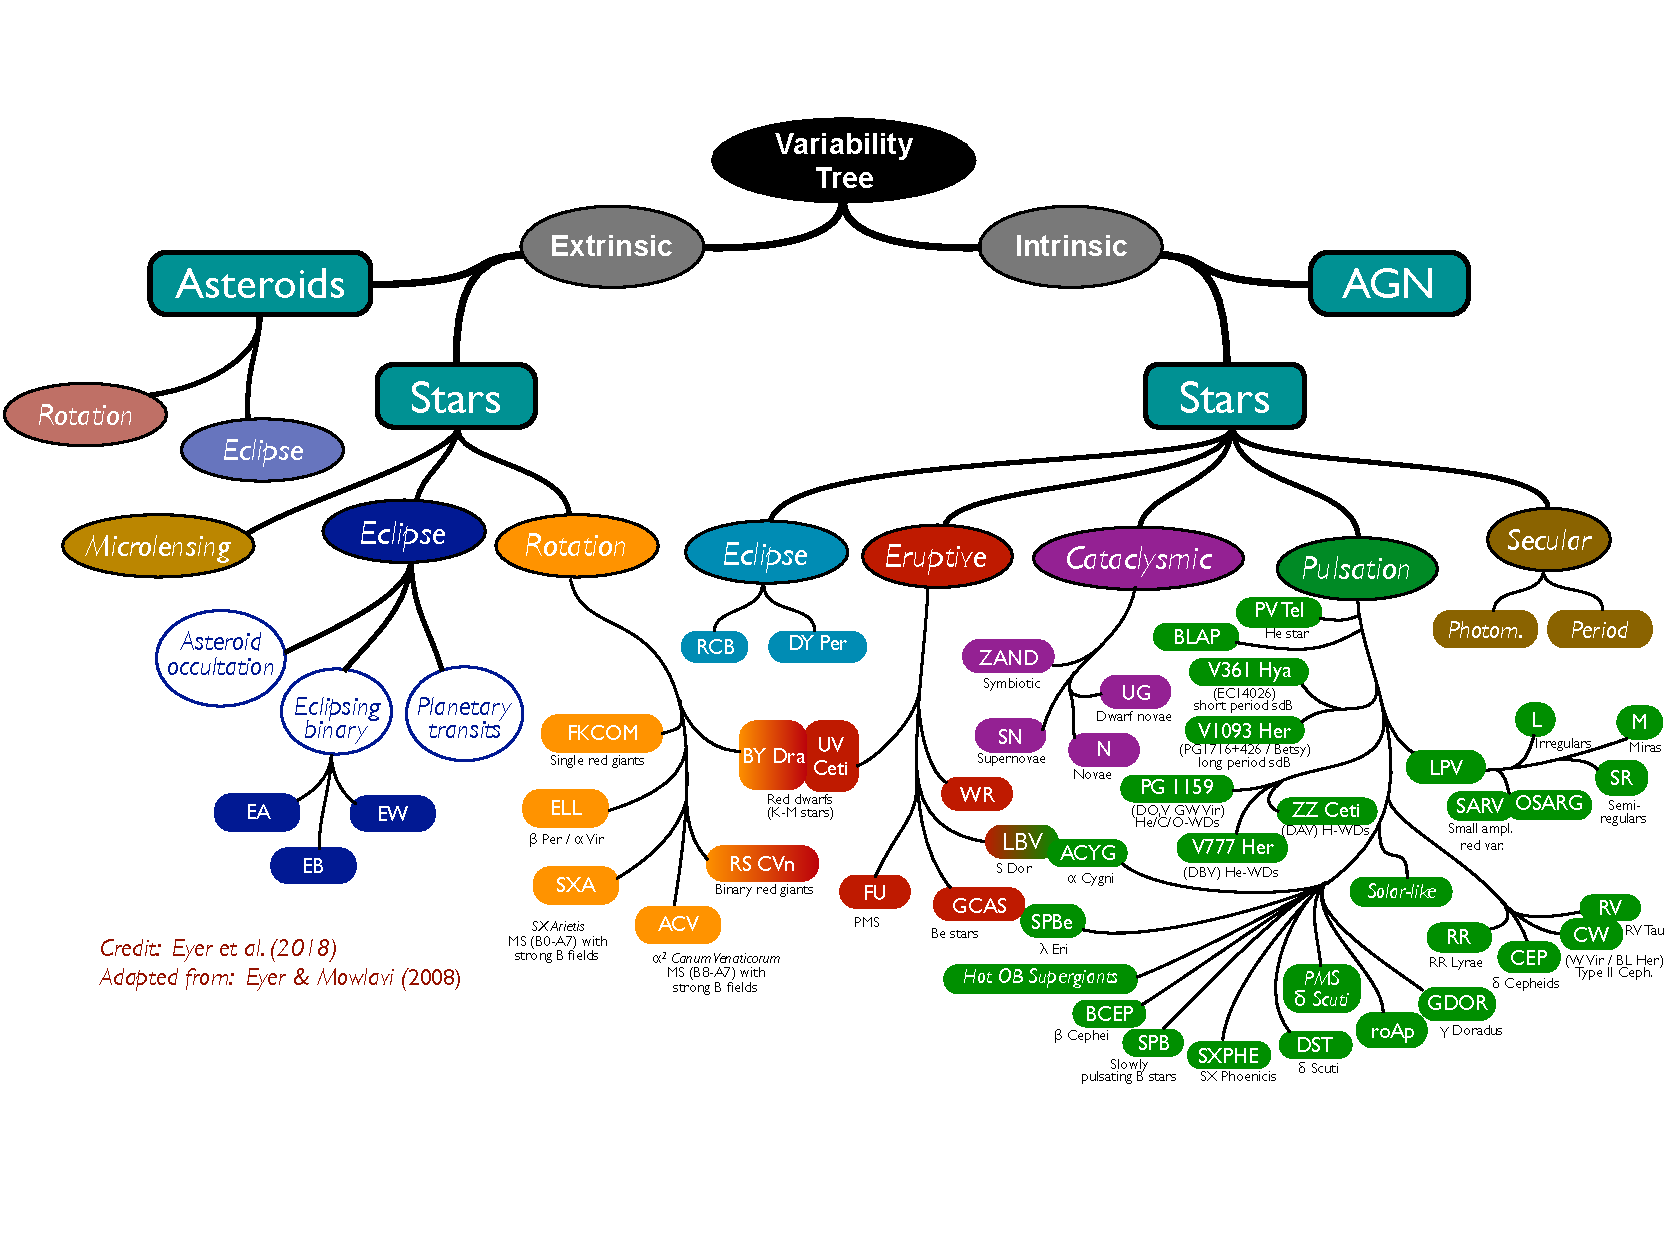
\includegraphics[width=1\linewidth]{04_antecedentes/figures/classification.pdf}
    \caption{
       Árbol de variabilidad. Expone en detalle la organización de objetos variables. Crédito: \citet{eyer2019gaia}. 
    }
    \label{fig:classification}
\end{figure}

En las variables extrínsecas, los cambios de brillo son el producto de ocurrencias externas, como pueden ser las interacciones de la estrella con otros cuerpos celestes o los efectos de su rotación estelar. Un caso característico de las extrínsecas son las estrellas eclipsantes \citep{wood1956eclipsingvariables}, que forman parte de sistemas binarios. En estos sistemas, dos estrellas orbitan alrededor de un centro de masa común y, desde la perspectiva de la Tierra, una de ellas pasa periódicamente frente a la otra, aparentando una disminución en el brillo observado.

En contraste, las variables intrínsecas deben su variabilidad a procesos físicos internos que acaban alterando la propia luminosidad de la estrella, como las pulsaciones radiales en sus capas externas o eventos eruptivos en su superficie. En el caso de las estrellas pulsantes \citep{cox1974pulsatingvariables}, por ejemplo, la variación periódica de la luminosidad se debe a ciclos regulares de expansión y de contracción en las capas más externas de la estrella. Impulsadas por la interacción entre la presión y la gravedad, estas oscilaciones producen una relación directa entre la luminosidad del objeto y su período de pulsación: la llamada ley período-luminosidad \citep{leavitt1912periods}. Esta relación hace que las estrellas pulsantes sean objetos de estudio especialmente interesantes, porque las convierte en herramientas valiosas para la determinación precisa de distancias en el universo.

\section{El papel de las estrellas variables pulsantes en la estimación de distancias}

La relación período-luminosidad, descubierta por Henrietta Swan Leavitt \citep{leavitt1907variables, leavitt1912periods}, establece que las variables pulsantes con un período de pulsación más largo son, en general, más luminosas. Este principio cobra importancia en dos tipos de estrellas pulsantes particulares:

\begin{description}
    \item[Las \emph{Cepheid}]
    Son gigantes o supergigantes cuya relación período-luminosidad ha sido calibrada con alta precisión, especialmente mediante observaciones en cúmulos cercanos y con instrumentos como el \emph{Hubble Space Telescope} \citep{altavilla2004cepheids}. A partir de su período de pulsación, se obtiene la luminosidad intrínseca de la estrella la cual, comparada con el brillo observado permite calcular su distancia. La alta luminosidad de las \emph{Cepheid} las hace especialmente útiles para medir distancias extragalácticas.
    
    \item[Las \emph{RR Lyrae}]
    Estas estrellas más pequeñas y antiguas, comunes en cúmulos globulares y el halo galáctico \citep{dallora2006rrlyraedistancescale}, tienen una luminosidad intrínseca menor, pero notablemente constante dentro de un rango de dispersión muy pequeño (particularmente en el filtro $V$). Esta estabilidad las convierte en marcadores confiables (candelas estándar) para medir distancias en escalas galácticas y locales, como dentro de la Vía Láctea y sus cúmulos asociados. 
\end{description}

Tanto las \emph{Cepheid} como las \emph{RR Lyrae} son utilizadas en la aproximación de distancias cósmicas, proporcionando un vínculo entre mediciones locales y estructuras a mayor escala. Su luminosidad intrínseca, comparada con su brillo observado, permite calcular el módulo de la distancia mediante la ecuación
\[
m - M = 5 \log_{10}(\frac{d}{\SI{10}{pc}})
\]
donde $d$ es la distancia en pársecs, $M$ es la magnitud absoluta y $m$ la magnitud aparente. Aunque esta relación es especialmente útil en el estudio de estrellas variables, en realidad se puede aplicar a cualquier fuente cuya luminosidad intrínseca sea conocida.

La magnitud aparente es una medida del brillo que percibimos de un cuerpo celeste al ser observado desde la Tierra. Se mide con una escala logarítmica, en la que un número menor indica un objeto más brillante. La relación que se usa para la magnitud aparente es tal que una diferencia de magnitudes de 5 corresponde a un factor de 100 en el brillo observado, es decir, que una estrella de magnitud 1 es cien veces más brillante que una de magnitud 6.

Por otro lado, la magnitud absoluta indica el brillo que podríamos observar de un cuerpo celeste si estuviera ubicado a una distancia estándar de 10 pársecs (aproximadamente $32.6$ años luz). Es una propiedad intrínseca del objeto y está fuertemente relacionada con su luminosidad, la cantidad total de energía que emite por unidad de tiempo en todas las direcciones. Este valor depende de las características internas de la estrella, como su tamaño, temperatura y composición \citep{caroll2017astrophysics}.

\section{Curvas de luz}

El análisis detallado de una estrella variable comienza con su \acrfull{lc}, un gráfico que describe cómo varía el brillo de una estrella o una región celeste en función del tiempo. Se obtiene a partir de observaciones fotométricas repetidas, en las cuales se mide el brillo de un objeto celeste en diferentes momentos \citep{percy2007variablestars}. Las mediciones suelen expresarse en términos de magnitud aparente y contienen información sobre el tiempo de observación, típicamente en \glspl{jd}, es decir, la cantidad de días transcurridos desde el mediodía del 1º de enero del año 4713 a. C. También pueden incluir información adicional, como el nivel de incertidumbre.

Las \glspl{lc} pueden entenderse como una aplicación específica de las series temporales en astronomía que, en términos generales, son conjuntos de datos u observaciones ordenados cronológicamente con el fin de analizar la evolución de fenómenos a lo largo del tiempo \citep{richards2011timeseries}. Otros ejemplos de series temporales incluyen las variaciones diarias de temperatura, los índices bursátiles o las mediciones de tráfico en redes.

En algunos casos, resulta útil representar una \gls{lc} en función de la ``fase'' en lugar del tiempo absoluto. Esto se debe a que los tiempos de observación suelen estar distribuidos de forma irregular o aleatoria, lo que dificulta visualizar patrones periódicos en el tiempo cronológico. La fase se refiere a una medida del tiempo normalizada respecto al período de la estrella, indicando en qué punto del ciclo de variación se encuentra. Conociendo el período de la estrella observada, es posible plegar los datos en un intervalo de $[0,1)$, permitiendo visualizar la variabilidad periódica de manera más clara y comparativa entre diferentes ciclos.

\begin{figure}[!ht]
    \centering
    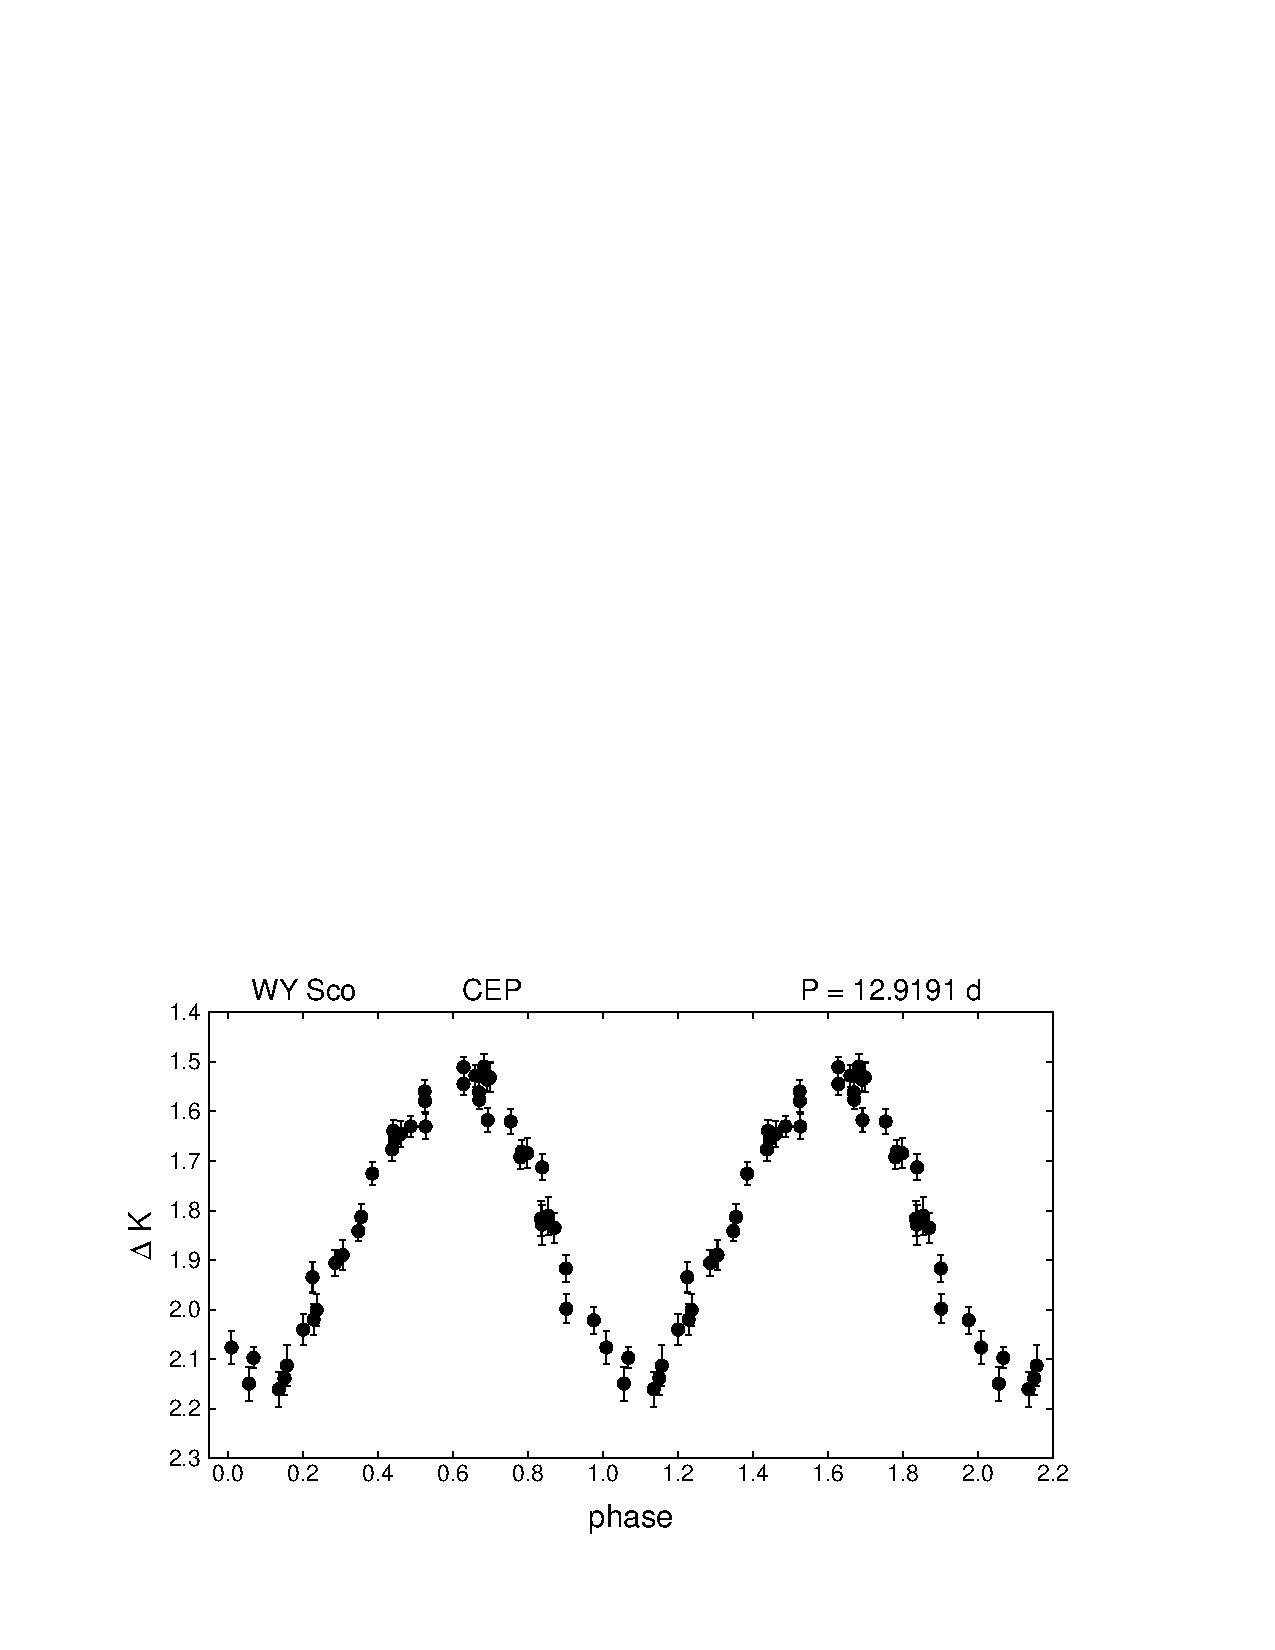
\includegraphics[width=0.8\textwidth]{04_antecedentes/figures/wys_opt.pdf}
    \caption{
       Observaciones de magnitud en la banda $K$ de la estrella \emph{Cepheid} WY Sco.
       El eje X representa la fase de medición. El eje Y, la magnitud en orden inverso.
       Crédito: \citet{catelan2011vvv}.
    }
    \label{fig:wys_opt}
\end{figure}


El gráfico de \autoref{fig:wys_opt} exhibe la \gls{lc} de una estrella \emph{Cepheid} puesta en fase. Los patrones regulares de aumento y disminución del brillo revelan el período de pulsación de la estrella. Además, la \gls{lc} expone detalles sobre la amplitud de los cambios de brillo, proporcionando información adicional sobre las propiedades físicas del objeto, como la masa y la composición química.
\section{El desafío de la era de los datos}

Con el advenimiento de nuevos telescopios y programas de observación, la astronomía ha ingresado en la era del \emph{Big Data}. Relevamientos masivos, como el \emph{Zwicky Transient Facility} \citep{bellm2018ztf}, tienen la capacidad de observar y monitorear millones de estrellas de manera continua y en múltiples bandas del espectro electromagnético, redefiniendo así los límites de la astronomía observacional y expandiendo nuestra comprensión del universo.

Uno de estos proyectos es el \acrfull{vvv} \citep{minniti2010vvv}, el cual hace uso del telescopio \gls{vista} ubicado en el Observatorio Paranal de Chile (\autoref{fig:vista}) para explorar el disco y el bulbo de la Vía Láctea en el infrarrojo cercano. Desde su inicio en 2010, el \gls{vvv} y su sucesor, el \gls{vvvx}, han llevado a cabo alrededor de 4200 horas de observación repartidas en un período de aproximadamente 13 años. En total, ha obtenido más de 350 mil imágenes, que componen un catálogo con más de $10^6$ archivos de observaciones \citep{saito2024vvvx}.

\begin{figure}[!ht]
    \centering
    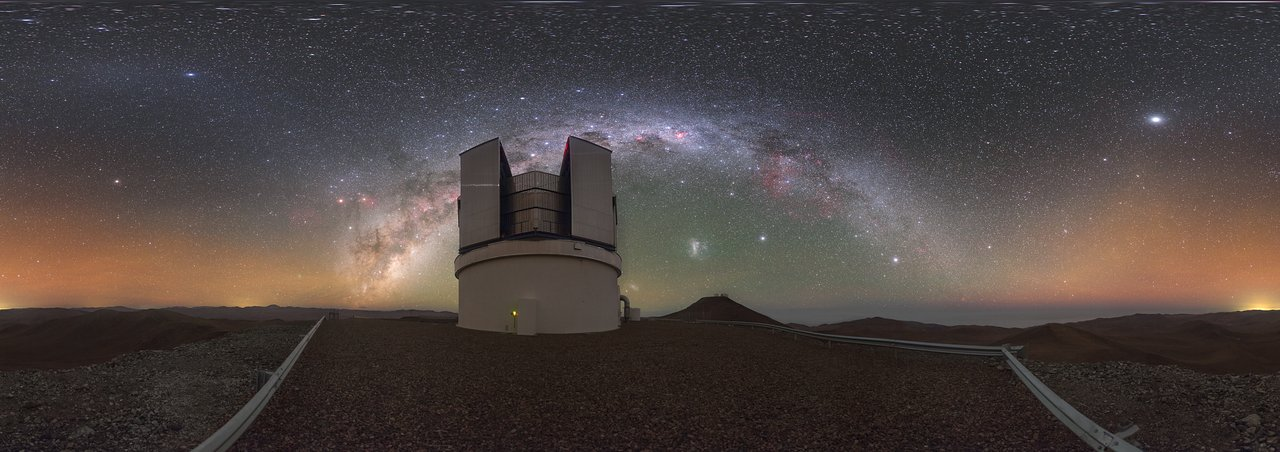
\includegraphics[width=0.8\textwidth]{04_antecedentes/figures/vista.jpg}
    \caption{
        El telescopio \acrfull{vista}, situado en el Observatorio Paranal de ESO, en Chile.
        Crédito: ESO/P. Horálek.
    }
    \label{fig:vista}
\end{figure}

Esta explosión de información no es exclusiva del \gls{vvv}. Proyectos similares como el futuro Observatorio Vera C. Rubin \citep{ivezi2019lsst} están preparados para producir volúmenes de datos aún mayores, presentando nuevos desafíos con respecto al manejo y análisis de estos datos en la astronomía moderna.

El creciente volumen y complejidad de los datos astronómicos hacen que el análisis manual de las observaciones sea inviable, volviendo indispensables el uso de nuevas técnicas automatizadas capaces de procesar información de manera eficiente. En este panorama, los algoritmos de \acrlongsp{ml} se han posicionado como herramientas clave para identificar patrones complejos que serían imposibles de detectar manualmente, abriendo nuevas puertas al conocimiento en una escala sin precedentes.


\section[Aprendizaje automático para la generación de conocimientos]{
    \Acrlongsp{ml} para la generación de conocimientos
}

El \acrfull{ml} es una rama de la inteligencia artificial que busca diseñar algoritmos capaces de aprender y mejorar a partir de datos, sin necesidad de reglas explícitas programadas. En términos simples, un programa se considera capaz de aprender si su desempeño en una tarea específica mejora con la experiencia \citep{mitchell1997machine}. Los algoritmos de \gls{ml} se pueden aplicar a grandes cantidades de datos para automatizar procesos complejos y mejorar la efectividad de tareas específicas, siendo las actividades de clasificación, regresión, optimización y agrupación las aplicaciones más comunes de los modelos de \gls{ml} \citep{michalski2013ml}.

El proceso por el cual se extrae conocimiento útil a partir de colecciones masivas de datos se denomina \gls{dm}. Esta técnica se apoya en gran medida en los algoritmos de \gls{ml} para identificar patrones y relaciones existentes entre los datos de manera automática y eficiente, lo que facilita el descubrimiento de información valiosa que de otro modo permanecería oculta.

Con el objetivo de sistematizar la generación de conocimiento a partir de volúmenes extensos de datos surge el método de \gls{kdd}. Inspirado en el método científico, \gls{kdd} define una serie de etapas secuenciales que buscan reducir la complejidad de los datos crudos para transformarlos en información útil y comprensible que puede ser utilizada para mejorar la toma de decisiones en diversos campos \citep{fayyad1996advances}. En la \autoref{fig:kdd} se aprecian las distintas etapas del proceso, que van desde la selección y el preprocesamiento de los datos hasta la interpretación y evaluación de los resultados.

\begin{figure}[!ht]
    \centering
    \makebox[\textwidth][c]{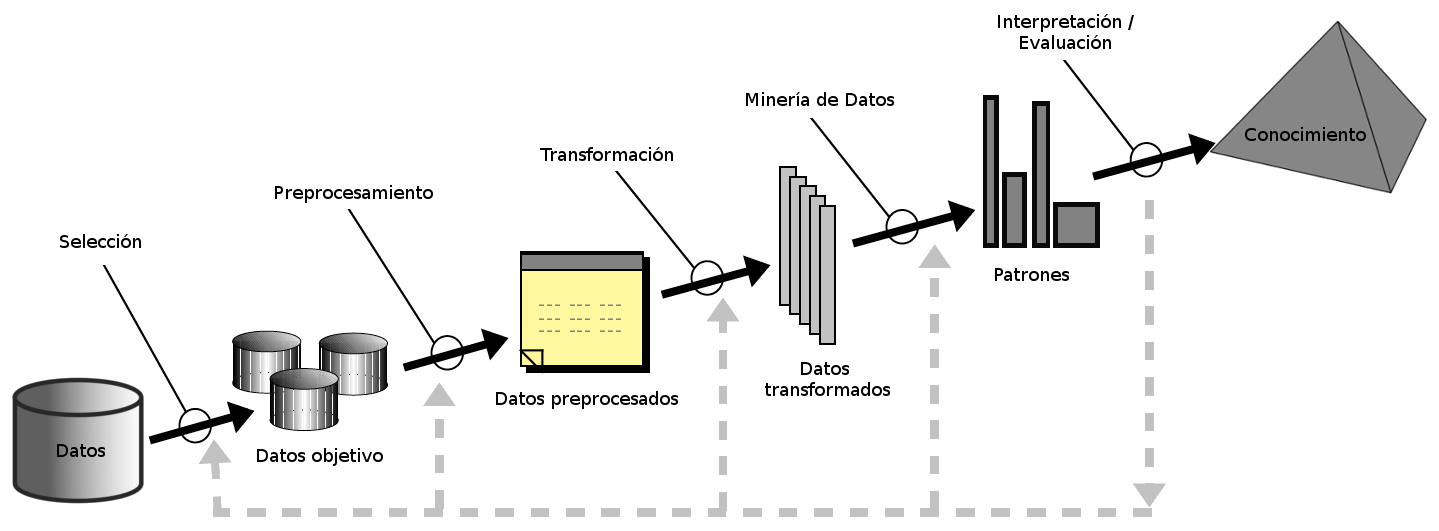
\includegraphics[width=1\linewidth]{04_antecedentes/figures/kdd.png}}
    \caption{
        Diagrama del procedimiento de KDD, adaptado de \citet{fayyad1996advances}.
    }
    \label{fig:kdd}
\end{figure}

El enfoque \gls{kdd} se sostiene principalmente en la fase de \gls{dm} como un puente entre los datos almacenados y el conocimiento. Si bien en la literatura es común utilizar los términos \gls{kdd} y \gls{dm} de manera intercambiable, en nuestro contexto hablaremos de \gls{dm} para referirnos específicamente a la etapa de identificación de patrones dentro del proceso completo de \gls{kdd}, el cual incluye las fases previas de preprocesamiento y transformación de los datos, así como la interpretación posterior de los resultados.

La efectividad de los algoritmos de \gls{ml} aplicados en la \acrlongsp{dm} está determinada por la calidad y representatividad de los datos que se utilicen como entrada. Las etapas de preprocesamiento y transformación son, entonces, fases especialmente importantes del enfoque \gls{kdd}, porque se encargan de limpiar y adaptar los datos crudos a una forma más fácil de manejar para los modelos de \gls{ml}. Este mecanismo no es automático; más bien, la naturaleza compleja de los datos hace que el proceso sea caro, tedioso y difícil, pues requiere de un conocimiento muy específico del dominio del problema para asegurar que los datos analizados son significativos.

En este trabajo nos enfocamos en la tarea de transformación de los datos para la reducción de complejidad y la identificación de atributos relevantes en los catálogos astronómicos. En particular, nos interesa la técnica de extracción de características, aplicada específicamente al estudio de \glspl{lc} para estrellas variables.

\section{Extracción de características}

Las \glspl{lc}, en su forma original como series temporales, constituyen datos de naturaleza inherentemente compleja y de alta dimensionalidad. Aunque contienen información valiosa sobre las propiedades físicas de las estrellas, esta se encuentra normalmente ofuscada por factores como la gran escala de los datos, el ruido instrumental y la incompletitud de las observaciones, haciendo del análisis de \glspl{lc} una tarea costosa incluso para los algoritmos avanzados de \gls{ml}.

Para abordar los problemas asociados a la complejidad de las \glspl{lc}, se emplea la técnica conocida como extracción de características \citep{khalid2014featureextraction}. Mediante este proceso, se transforman las series temporales originales en un conjunto de características clave que encapsulan la información más relevante para una representación más compacta y manejable de los datos.

Cuando hablamos de una característica, nos referimos a un descriptor cuantitativo que resume o representa algún aspecto importante del conjunto de datos. El conjunto completo de características define el llamado espacio de características, que conforma la representación final sobre la cual operan los modelos de \gls{ml}. Un espacio de características bien diseñado no solo reduce la carga computacional, sino que también mejora la capacidad del modelo para identificar patrones significativos, facilitando en nuestro caso tareas como la clasificación de estrellas variables y la predicción de parámetros físicos.

Las técnicas de extracción de características pueden involucrar tanto métodos manuales como automáticos. Los métodos automáticos se basan en técnicas de aprendizaje profundo como redes neuronales convolucionales \citep{chui2023convolutionalneuralnetwork} para derivar propiedades de manera implícita, partiendo únicamente de los datos; mientras que en los métodos manuales, en cambio, los investigadores definen explícitamente las características a calcular, seleccionando aquellas más relevantes en función del contexto.

Si bien los enfoques automáticos son útiles para identificar patrones en estructuras complejas, las características resultantes suelen ser limitadas en cuanto a su interpretabilidad, dificultando la comprensión física de los fenómenos. En contraste, el control que conceden los procesos manuales permite la extracción de propiedades con un significado físico claro, siendo este enfoque particularmente valioso en el panorama de \glspl{lc} al vincular las características extraídas con procesos observables. 

\section{Características de las curvas de luz}

En el análisis de \glspl{lc}, las características más efectivas son las que capturan las propiedades físicas de la estrella observada, como su periodicidad o su amplitud. Estas propiedades no solo son fácilmente interpretables, brindando información sobre los fenómenos subyacentes, sino que además simplifican la distinción entre los distintos tipos de estrellas variables. En el resto de esta sección, se detallan algunas de las características más relevantes de las \glspl{lc} empleadas en el análisis de estas estrellas.


\begin{description}
    \item[Período ($P$)]
    El período representa el tiempo que tarda una estrella variable en completar un ciclo completo de variación de brillo. Como ya dijimos, esta característica es especialmente conveniente en el caso de las \emph{Cepheid} y de las \emph{RR Lyrae}, porque posibilita el cálculo preciso de distancias astronómicas.
    
    El cálculo del período se realiza comúnmente mediante métodos espectrales como el de Lomb-Scargle \citep{lomb1976ls}, que identifica las frecuencias dominantes en los datos temporales. Siguiendo este método, el período se deriva como el inverso de la frecuencia principal:
    \[
    P = \frac{1}{f_{\max}}
    \]
    donde $f_{\max}$ es la frecuencia con mayor potencia en el espectro.

    \item[Amplitud ($A$)]
    Algunos tipos de estrellas pulsantes como las \emph{RR Lyrae} presentan amplitudes características en sus oscilaciones \citep{dallora2006rrlyraedistancescale}, por lo que se trata de una característica útil para clasificar las estrellas variables.
    
    La amplitud mide la diferencia entre el brillo máximo y mínimo registrado en la \gls{lc}. Por lo general, se suele considerar la mitad de esa diferencia con el fin de obtener una medida más representativa de la variación del brillo en torno al valor medio. La fórmula está dada por:
    
    \[
    A = \frac{\max{(m)} - \min{(m)}}{2}
    \]
    donde $m$ representa las magnitudes aparentes observadas.
    
    Cuando los datos contienen abundancia de ruido o de valores atípicos, se puede emplear un cálculo de la amplitud más robusto que considera las medianas del $5\%$ superior e inferior de las magnitudes observadas, en lugar de los máximos y mínimos absolutos \citep{richards2011timeseries}.
    
    \item[\emph{Skewness} ($G_1$)]
    El \emph{skewness} es una medida de la asimetría en la distribución de las magnitudes en una \gls{lc}. Matemáticamente, se define como:
    
    \[
    G_1 = \frac{N}{(N - 1)(N - 2)} \frac{\sum_i(m_i - \bar{m})^3}{\sigma_m^3},
    \]
    donde $N$ es el número de observaciones, $\bar{m}$ es la media muestral de la magnitud y $\sigma_m$ es la desviación estándar muestral \citep{joanes1998skewnesskurtosis}.
    
    Un valor positivo de asimetría indica una curva con un ascenso lento y un descenso rápido, mientras que un valor negativo indica lo opuesto. Esta característica es de utilidad para identificar la forma de las oscilaciones en estrellas pulsantes.
\end{description}

Además de las características ya mencionadas, existen otras propiedades estadísticas y dinámicas que enriquecen aún más el análisis de las \glspl{lc}. Algunas de estas, utilizadas por \citet{richards2011timeseries} en su trabajo para la clasificación de estrellas variables, son:
\begin{itemize}
    \item \emph{Frecuencia}: Relacionada con el período, indica la cantidad de ciclos por unidad de tiempo.
    \item \emph{Autocorrelación}: Evalúa la similitud entre diferentes puntos de la curva.
    \item \emph{Índice de variabilidad}: Mide la variabilidad global de la \gls{lc}, proporcionando una estimación cuantitativa de las fluctuaciones de brillo a lo largo del tiempo.
    \item \emph{Kurtosis}: Medición de la ``altitud'' y la ``anchura'' de los picos de la curva. Proporciona información sobre la concentración y la dispersión de los datos.
\end{itemize}

\section{Cómputo distribuido}

El volumen y complejidad de los datos astronómicos no sólo desafían nuestra capacidad de análisis, sino también las infraestructuras computacionales que los sustentan. A medida que la cantidad de datos a analizar sigue creciendo de manera exponencial, los sistemas tradicionales de procesamiento centralizado ya no son suficientes para enfrentar los desafíos de escalabilidad, eficiencia y rapidez que demandan las aplicaciones modernas. En este contexto, el cómputo distribuido proporciona una solución viable para paralelizar el preprocesamiento de datos \citep{zaharia2016stark}, el entrenamiento de modelos de \gls{ml} \citep{dean2012distributeddeepnetworks} y la ejecución de análisis en múltiples nodos \citep{abadi2016tensorflow}.

El concepto de cómputo distribuido se refiere a un paradigma de procesamiento en el que múltiples máquinas (o nodos) trabajan conjuntamente para resolver una tarea que no podría ser procesada de manera eficiente en un solo sistema \citep{tanenbaum2006distributedsystems, coulouris2011distributedsystems}. En este enfoque, los recursos de varios dispositivos, a menudo dispersos geográficamente y conectados por una red, se agrupan para ejecutar programas de manera colaborativa. Cada nodo en un sistema distribuido puede tener su propia memoria y CPU, y todos operan de forma coordinada, a menudo compartiendo información y procesando partes de un mismo problema en paralelo.

En términos de la estructura física de los sistemas, el concepto de cómputo distribuido no es una novedad, pues la idea de distribuir el trabajo entre varios equipos de computación se viene implementando desde hace varias décadas. Sin embargo, la reciente expansión del acceso a redes de alta velocidad y la mejora en la capacidad de los sistemas de comunicación han acelerado su adopción \citep{kurose2012networks}.

\section{Paralelismo y concurrencia}

Dentro de la construcción de sistemas de cómputo distribuidos, el paralelismo y la concurrencia representan bloques fundamentales para aprovechar al máximo los recursos disponibles del sistema \citep{silberschatz2012operatingsystems}. Mientras que el cómputo distribuido se encarga de coordinar múltiples nodos para abordar una tarea de gran escala, el paralelismo y la concurrencia se ocupan de explotar la capacidad interna de cada nodo, dividiendo el trabajo entre los múltiples núcleos de procesamiento que lo componen.

El paralelismo refiere a la ejecución simultánea de tareas. Esta técnica consiste en dividir un problema grande en varios subproblemas que puedan ser resueltos de forma independiente y en paralelo por diferentes unidades de cómputo. El objetivo es maximizar la utilización de los recursos disponibles, ya sean los núcleos de CPU o los nodos de una red distribuida, para acortar los tiempos de ejecución. Existen dos formas comunes de paralelismo:

\begin{itemize}
    \item \emph{Paralelismo de datos}. Se aplica la misma operación sobre diferentes conjuntos de datos en paralelo. Por ejemplo, entrenar un modelo de \gls{ml} sobre un \emph{data set} dividido \citep{dean2012distributeddeepnetworks}.
    
    \item \emph{Paralelismo de tareas}. Se ejecutan operaciones diferentes sobre un mismo conjunto de datos. Un caso típico
    es el procesamiento de imágenes, donde las operaciones disponibles son independientes entre sí \citep{saxena2016imageprocessing}.

\end{itemize}

Por otro lado, la concurrencia apunta a la gestión de múltiples tareas que progresan de forma simultánea, aunque no necesariamente se ejecuten exactamente al mismo tiempo. A menudo, la concurrencia se implementa para permitir que un programa realice operaciones mientras espera otras más lentas, como accesos a disco o llamadas de red, garantizando que ninguna tarea se quede estancada \citep{mccool2012parallel}.

En el ámbito de la programación, las ideas de paralelismo y concurrencia suelen implementarse mediante dos estrategias comunes:

\begin{description}
    \item[\emph{Multithreading}] (``multihilos'') 
    Se basa en el uso de múltiples hilos (\emph{threads}) de ejecución compartiendo un mismo espacio de memoria. Es una estrategia eficaz para programas que realizan muchas operaciones de entrada y salida, ya que permite que el sistema avance mientras espera la finalización de tareas bloqueantes.
    
    Los interpretes comunes de Python implementan un \gls{gil} que limita la ejecución concurrente de código Python puro, lo que restringe su efectividad en tareas intensivas de CPU \citep{piñeiro2024omp4pypurepythonimplementation}.

    \item[\emph{Multiprocessing}] (``multiprocesamiento'')
    Mediante esta técnica, se crean múltiples procesos aislados que no comparten memoria. A diferencia de los hilos, estos procesos sí pueden ejecutarse verdaderamente en paralelo, incluso sobre múltiples núcleos físicos, por lo que resulta especialmente útil cuando las tarea son independientes entre sí. En contraste, esta estrategia se ve comprometida cuando hay mucha comunicación entre procesos, pues presenta una mayor sobrecarga al no compartir una memoria.
 
    La separación de procesos permite que cada uno cuente con su propia instancia del intérprete de Python, sorteando así las limitaciones impuestas por el \gls{gil}.
\end{description}

La elección entre \emph{multithreading} y \emph{multiprocessing} depende de la naturaleza del problema, así como del entorno de ejecución. Como el \emph{multithreading} puede verse limitado por el \gls{gil}, suele emplearse cuando el problema involucra muchas operaciones de entrada y salida, mientras que las técnicas de \emph{multiprocessing} son más adecuadas cuando las tareas requieren alto poder de procesamiento y no necesitan compartir datos entre sí. En resumen: si el cuello de botella es la CPU, es preferible el \emph{multiprocessing}; si es la latencia de operaciones de I/O, \emph{multithreading} \citep{bienia2008parsec}. Entender estas distinciones resulta fundamental para desarrollar soluciones escalables y eficientes en contextos de análisis de datos de gran escala.


\section[Olores en el código: de FATS a feets]{
    Olores en el código: de \acrshort{fats} a \acrshort{feets}
}


\gls{fats} \citep{nun2015fatsfeatureanalysistime} es una herramienta diseñada para la extracción de características a partir de series temporales, particularmente de \glspl{lc} de objetos variables. Construida sobre el \emph{stack} científico de Python\footnote{\url{https://www.python.org/}}, \gls{fats} proporciona un \emph{framework} estandarizado que incluye extractores de características listos para usar, así como permite el desarrollo de nuevos extractores de manera flexible.

A pesar de las utilidades ofrecidas por \gls{fats}, su diseño e implementación han presentado diversas limitaciones que, a la larga, condujeron al desarrollo de su sucesor, \gls{feets}. Estas deficiencias se ven evidenciadas por la presencia de ``malos olores'' en el código, o \emph{code smells}.

Según \citet{fowler2006codesmell}, se les dice \emph{code smells} a
\begin{quote}
    ...indicios superficiales en el código que sugieren problemas más profundos en el sistema...
\end{quote}

En el caso de \gls{fats}, el análisis en profundidad de estos \emph{code smells} \citep{cabral2018fatsfeetsimprovementsastronomical} llevó a la identificación de varias problemáticas significativas como el uso de variables globales, la gestión inadecuada de errores y la implementación de código no estandarizado. Estos problemas, sumados a la falta de documentación y a la incompatibilidad con nuevas versiones de Python, impactaron negativamente en la usabilidad de la herramienta.

En respuesta a las limitaciones identificadas en \gls{fats} se llevó a cabo el desarrollo de una nueva herramienta, \acrfull{feets} \citep{cabral2018feets}. Este proyecto implicó una reingeniería completa de \gls{fats}, reestructurada para resolver los problemas clave detectados y agregar otras mejoras significativas, incluyendo avances como la eliminación de variables globales y la optimización de algoritmos para un mejor rendimiento. Además, \gls{feets} incluye una documentación detallada y posee una cobertura de pruebas del 90\%, garantizando un \emph{software} más robusto, accesible y confiable para la comunidad astronómica.

La transición de \gls{fats} a \gls{feets} se centró en mejorar el diseño y la arquitectura de la herramienta sin modificar sus funcionalidades principales, un proceso comúnmente conocido como refactorización de código. Este enfoque permite modificar el diseño interno del \emph{software} para mejorar su calidad, mientras se mantienen los resultados esperados para los usuarios finales.

\section{Refactorización y calidad de \emph{software}}

La refactorización de código, formalizada por \citet{fowler1999refactoring}, es un proceso en la ingeniería del \emph{software} orientado a mejorar la estructura interna del código sin alterar su comportamiento externo. El objetivo principal de la refactorización es mejorar la comprensión del código y su adaptación a futuros cambios.

Este proceso no se reduce a una sola técnica, sino que comprende un conjunto de varias prácticas que, en conjunto, mejoran el diseño del código. Por ejemplo, dividir funciones extensas en subfunciones más específicas aumenta la claridad del código y permite desarrollar pruebas más efectivas. Del mismo modo, adoptar nombres precisos para las variables, métodos y clases ayuda a mejorar su interpretación y mantenimiento \citep{martin2009clean}.

Más allá de la claridad y la organización del código, la refactorización impacta directamente en la calidad del \emph{software} \citep{kaur2017qualityrefactoring}. Un código bien estructurado no solo facilita su mantenimiento, sino que también influye en atributos clave que determinan su fiabilidad y sostenibilidad a largo plazo.

La calidad del \emph{software} se entiende como el grado en que un sistema, componente o proceso cumple con los requisitos especificados y las expectativas del usuario \citep{iso9126quality}. El concepto de calidad se asocia principalmente a la correcta funcionalidad del sistema y a su conformidad con los requerimientos, pero también abarca atributos no funcionales que son fundamentales para su sostenibilidad y evolución. Por ejemplo:
\begin{itemize}
    \item \emph{Mantenibilidad}: La capacidad de ser modificado fácilmente, ya sea para corregir defectos, mejorar su rendimiento o adaptarlo a nuevos requerimientos.

    \item \emph{Eficiencia}: El uso adecuado de los recursos del sistema, como el tiempo de procesamiento, la memoria y otros recursos computacionales.

    \item \emph{Usabilidad}: La facilidad con la que los usuarios pueden interactuar con el sistema.

    \item \emph{Escalabilidad}: La capacidad para manejar un aumento en la carga de trabajo o el volumen de usuarios sin degradar su rendimiento.
\end{itemize}
La refactorización, al mejorar la estructura y diseño interno del código, contribuye directamente a potenciar estos aspectos, esenciales para el desarrollo de \emph{software} robusto y adaptable.

\section{Principios para el diseño de \emph{software}}

El diseño de \emph{software} se refiere al proceso de definir la arquitectura y estructura de un sistema, así como la organización de sus componentes y las formas que interactúan entre sí. Un buen diseño debe buscar que el \emph{software} sea fácil de interpretar, mantener y extender a lo largo del tiempo.

Respaldadas por el principio básico ``divide y vencerás'', las estrategias comunes de diseño consisten en dividir un sistema complejo en componentes más pequeñas, fáciles de manipular. Aunque estas partes no son independientes, su separación facilita la cooperación entre sí dentro de una jerarquía organizada. Esta partición busca que cada componente pueda entenderse, implementarse y mantenerse de forma individual, lo que reduce la complejidad global del sistema como un todo \citep{martin2003agilesoftwaredevelopment}.

Para lograr la separación efectiva de responsabilidades, resulta esencial contar con una buena abstracción: una descripción del comportamiento externo de un componente que oculta sus detalles internos. La correcta implementación de estos aspectos da lugar a un diseño modular \citep{parnas1972modularization}, separado en unidades discretas que pueden ser diseñadas, implementadas, probadas y modificadas con facilidad, manteniendo un impacto mínimo (o nulo) sobre las demás partes del sistema. Para lograr una modularidad efectiva, el diseño debe considerar dos propiedades importantes: el acoplamiento y la cohesión de los módulos \citep{jalote1997integrated}.

\begin{description}
    \item[El acoplamiento] es un concepto intermodular que captura la noción de dependencia entre módulos. Dos módulos son independientes si cada uno puede funcionar completamente sin la presencia del otro. Cuanto mayor es la dependencia entre módulos, mayor es la complejidad de las interfaces, por lo que se desea reducir el acoplamiento lo más que se pueda. En lenguajes como Java\footnote{\url{https://docs.oracle.com/en/java/index.html}}, una alta cantidad de sentencias \texttt{import} puede ser un indicio de acoplamiento excesivo, ya que refleja una fuerte dependencia del módulo respecto de múltiples componentes externos.
    
    \item[La cohesión] caracteriza, en cambio, el vínculo intramodular, es decir la relación entre los elementos dentro de un módulo. Un módulo con alta cohesión realiza actividades muy relacionadas entre sí, mientras que uno con cohesión baja intenta abarcar varias responsabilidades distintas. Por lo general se busca que un módulo se encargue de una sola tarea específica, por lo que es deseable conservar una cohesión elevada. Un indicador de cohesión es la relación entre estado y comportamiento: si la mayoría de los métodos de un módulo accede a sus atributos privados, esto sugiere que el estado interno está bien integrado con su funcionalidad.
\end{description}

\subsection{SOLID para el diseño orientado a objetos}

En el diseño de \emph{software} no existe un conjunto rígido de pasos que garantice el éxito, pero sí existen principios fundamentados en la ingeniería del \emph{software} que guían el proceso de diseño hacia soluciones robustas, escalables y de alta calidad.

Los principios SOLID \citep{martin2000design}, por ejemplo, son un conjunto de cinco principios diseñados específicamente para la programación orientada a objetos. Constituyen una serie de prácticas que mejoran la estructura y la calidad del código para alinearlo a las propiedades de un buen diseño. Cada una de las siglas de SOLID representa un principio distinto:

\begin{enumerate}
    \item \emph{S -- Principio de Responsabilidad Única (SRP)}.
    Una clase debe tener una única razón para cambiar, es decir, debe ser responsable de una sola funcionalidad dentro del sistema.

    \item \emph{O -- Principio de Abierto-Cerrado (OCP)}.
    Los objetos o entidades debe estar abierto para su extensión pero cerrado para su modificación.

    \item \emph{L -- Principio de Sustitución de Liskov (LSP)}.
    Las clases derivadas deben poder sustituir a sus clases base sin alterar el comportamiento del sistema \citep{liskov1994subtyping}.

    \item \emph{I -- Principio de Segregación de Interfaces (ISP)}.
    Un cliente no debe implementar una interfaz que no utilice, ni debe depender de métodos que no use. Es preferible definir múltiples interfaces pequeñas y especializadas antes que una interfaz grande y genérica.
    
    \item \emph{D -- Principio de Inversión de Dependencias (DIP)}.
    Las módulos de alto nivel no deben depender de módulos de nivel más bajo, sino de abstracciones.
\end{enumerate}

\section{Algunos patrones de diseño}

A lo largo del tiempo, los desarrolladores han identificado soluciones recurrentes a problemas comunes en la arquitectura del \emph{software}, dando origen a los patrones de diseño. Estos patrones ofrecen soluciones estandarizadas para problemas específicos en la estructuración y comportamiento del sistema \citep{gamma1995designpatterns, shvets2018dive}. No son fragmentos de código listos para copiar y pegar, sino estructuras y principios que guían el diseño de soluciones eficaces. A continuación, exploraremos algunos de los patrones de diseño que fueron relevantes para la orquestación de este proyecto.

\subsection{Patrón \emph{Template Method}}

El patrón \emph{Template Method} define la estructura de un algoritmo complejo en una clase base y delega la implementación de pasos específicos a sus distintas subclases, permitiendo su personalización sin modificar la estructura general del algoritmo \citep{shvets2018dive}. Este enfoque permite reutilizar lógica común y adaptar su comportamiento en función de las necesidades de las distintas clases, garantizando la coherencia en la ejecución.

\begin{figure}[!ht]
    \centering
    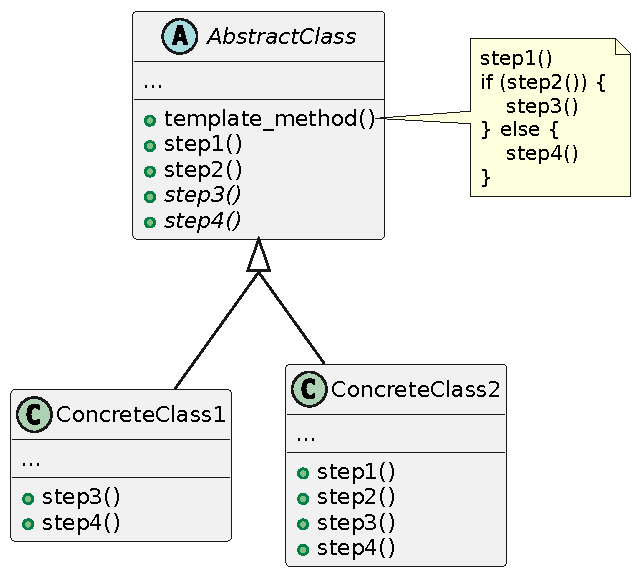
\includegraphics[width=0.55\textwidth]{04_antecedentes/figures/patterns/template_method.pdf}
    \caption{
        Diagrama UML que define el patrón \emph{Template Method}, extraído de \citet{shvets2018dive}. Los métodos abstractos se denotan por el uso de itálicas.
    }
    \label{fig:patterns/template_method}
\end{figure}

Como lo ilustra la \autoref{fig:patterns/template_method}, el patrón separa la estructura en dos tipos de clases:

\begin{description}
    \item[Una clase abstracta] (\texttt{AbstractClass}), que divide un algoritmo complejo en una serie de pasos, cada uno encapsulado en un método separado (\texttt{step1()}, \texttt{step2()}, \texttt{step3()} y \texttt{step4}()), y los integra ordenadamente dentro de un método de más alto nivel, el llamado ``\emph{template method}'' (\texttt{tem\-plate\_me\-thod()}).

  \item[Las subclases concretas] (\texttt{ConcreteClass1} y \texttt{ConcreteClass2}), que pueden reimplementar todos los pasos, pero sin alterar la lógica del \emph{template method}.
\end{description}

Algunos de los pasos individuales pueden ser abstractos, obligando a las subclases a proveer la implementación de su método correspondiente, mientras que los otros pueden ser opcionales, con una implementación predeterminada en la clase base, común para todas las subclases.

Para dar un ejemplo concreto, supongamos que queremos crear una aplicación destinada al análisis de documentos. Se espera que la aplicación funcione para distintos tipos de archivo (PDF, CSV y JSON), y que se pueda extender fácilmente a nuevos formatos si así se requiere. Después de analizar el problema, se redujo el proceso de análisis a cuatro etapas puntuales: \begin{enumerate}
    \item abrir el archivo que se desea analizar en modo de lectura
    \item extraer el texto del archivo
    \item procesar los datos extraídos
    \item generar un reporte con los resultados del análisis 
\end{enumerate}

\begin{figure}[!ht]
    \centering
    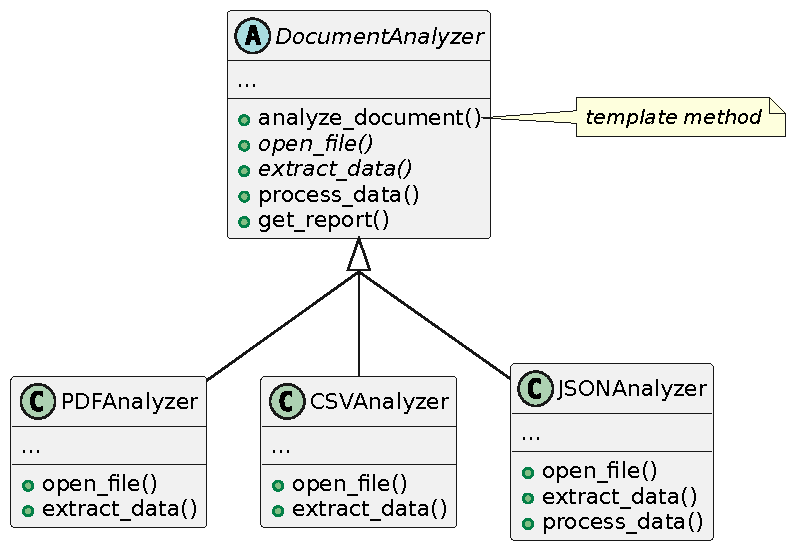
\includegraphics[width=0.725\textwidth]{04_antecedentes/figures/patterns/template_method_example.pdf}
    \caption{
        Diagrama UML del ejemplo del analizador de documentos, siguiendo el patrón \emph{Template Method}. Los métodos abstractos se denotan por el uso de itálicas.
    }
    \label{fig:patterns/template_method_example}
\end{figure}

Aplicando el patrón \emph{Template Method}, es posible llegar a un diseño como el de la \autoref{fig:patterns/template_method_example}.
La clase abstracta \texttt{DocumentAnalyzer} define el comportamiento del método \texttt{analyze\_document()} que funciona como un \emph{template method} para llevar a cabo el proceso completo de análisis. El algoritmo está separado en cuatro métodos diferentes, uno para cada paso identificado: \texttt{open\_file()}, \texttt{extract\_data()}, \texttt{process\_data()} y \texttt{get\_report()}.

Las subclases \texttt{PDFAnalyzer}, \texttt{CSVAnalyzer} y \texttt{JSONAnalyzer} implementan la lógica específica para el análisis de PDF, CSV y JSON respectivamente. Se determinó que los pasos de apertura de archivos y de extracción son muy dependientes del tipo de archivo analizado, por lo que sus métodos correspondientes se definen como abstractos, mientras que la lógica detrás del procesamiento y de la generación del reporte es muy similar para los distintos formatos de archivo, por lo que sus métodos constan de una implementación predefinida en la clase base.

\subsection{Patrón \emph{Facade}}

El patrón \emph{Facade} hace uso de una clase que proporciona una interfaz simplificada a un subsistema más complejo, actuando como una ``fachada''. De esta forma, reduce la dependencia de los clientes con las diferentes partes del subsistema.

Una fachada puede limitar las funcionalidades de los subsistemas a solo aquellas que requieran los clientes. Puede ser útil, por ejemplo, al querer integrar una aplicación con una biblioteca que provea decenas de funcionalidades, de las cuales solo se necesitan algunas pocas para solucionar el problema en cuestión.

\begin{figure}[!ht]
    \centering
    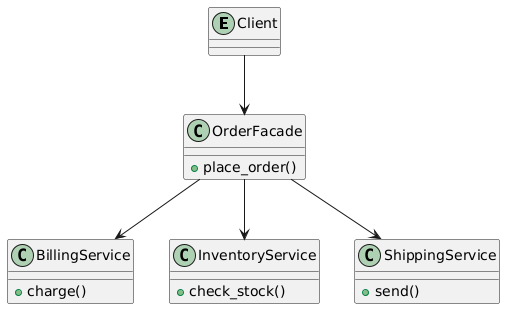
\includegraphics[width=0.75\textwidth]{04_antecedentes/figures/patterns/facade.png}
    \caption{
        Diagrama UML que define el patrón \emph{Facade}, extraído de \citet{shvets2018dive}.
    }
    \label{fig:patterns/facade}
\end{figure}

La \autoref{fig:patterns/facade} exhibe la estructura del patrón \emph{Facade}, que típicamente consiste de las siguientes partes:

\begin{description}
    \item[Una clase fachada] (\texttt{Facade}) que proporciona una interfaz conveniente para acceder a funcionalidades específicas del subsistema. Conoce cómo operar con las distintas partes del subsistema, y a dónde redirigir las solicitudes del cliente.

    \item[Otras fachadas] (\texttt{AdditionalFacade}) que pueden ser opcionalmente creadas para evitar tener una sola fachada con varias funcionalidades no relacionadas, reduciendo su complejidad. Estas fachadas adicionales pueden ser utilizadas tanto por el cliente como por las otras fachadas.

    \item[El subsistema complejo] (\texttt{ComplexSubsystem}) con múltiples componentes que proveen distintas funcionalidades. Normalmente, uno tendría que involucrarse con los detalles de implementación del subsistema para poder utilizar sus funcionalidades de la forma correcta. Las clases del subsistema (\texttt{SubsystemClass1}, \texttt{SubsystemClass2}, etc.) no deberían ser conscientes de la existencia de la fachada, sino que se comunican directamente entre sí sin operar por fuera del subsistema.

    \item[El cliente] que hace uso de la fachada sin hacer llamadas directas al subsistema.
\end{description}

Pongamos como ejemplo una aplicación de gestión de pedidos, que cuenta con servicios internos que se ocupan de distintas tareas: facturación, inventario y envío. La \autoref{fig:patterns/facade_example} visualiza el uso del patrón \emph{Facade} para tal ejemplo, donde la aplicación se comunica directamente con la clase \texttt{OrderFachade} que actúa como una fachada para ordenar la comunicación con las funcionalidades respectivas de los distintos servicios (\texttt{BillingService}, \texttt{InventoryService} y \texttt{ShippingService}).

\begin{figure}[!ht]
    \centering
    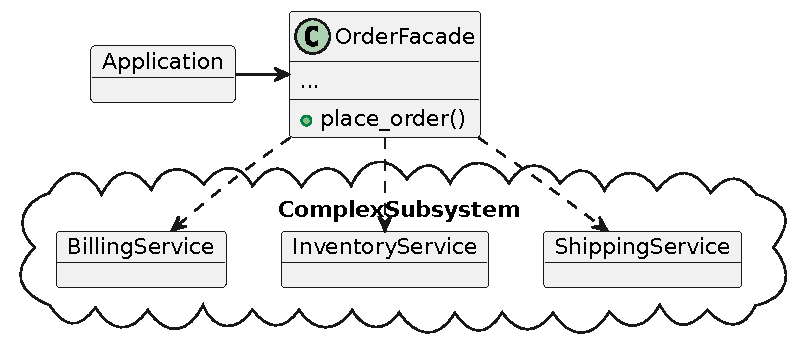
\includegraphics[width=0.75\textwidth]{04_antecedentes/figures/patterns/facade_example.pdf}
    \caption{
        Diagrama UML del ejemplo del gestor de pedidos siguiendo el patrón \emph{Facade}.
    }
    \label{fig:patterns/facade_example}
\end{figure}

\section{Métricas de calidad}

Empleando análisis estático sobre el código fuente de un sistema, es posible obtener ciertas métricas cuantitativas para estimar una noción objetiva de su calidad. La aplicación sistemática de estas métricas permite priorizar las áreas más problemáticas y enfocar los esfuerzos de refactorización donde se necesiten con mayor urgencia \citep{chidamber1994metrics, fowler1999refactoring}. A continuación, se describen las métricas más relevantes para los fines de este trabajo.

\subsection[Complejidad ciclomática (CC, Cyclomatic Complexity)]{
    \Gls{cc}
}

La \acrlongsp{cc}, propuesta por \citet{mccabe1976complexity}, mide la cantidad de caminos linealmente independientes en el flujo de control de un programa. Se suele usar este valor como una representación de la dificultad para entender, probar y mantener el código.

Se calcula a partir del grafo de flujo de control del programa con la siguiente fórmula:
\[
\text{CC} = E - N + 2P
\]
en donde:

\begin{align*}
    E&: \text{Número de aristas (conexiones entre nodos),} \\
    N&: \text{Número de nodos (bloques de código), y} \\
    P&: \text{Número de componentes conectados (p. ej.: funciones o métodos).}
\end{align*}

Un valor alto de \gls{cc} indica que el código tiene demasiadas bifurcaciones, lo que dificulta su mantenimiento. Idealmente, debería tener un valor menor a 10 para cada función o método.

\subsection{Métricas de Halstead}

Las métricas de Halstead \citep{halstead1977metrics} evalúan propiedades cuantitativas del código relacionadas con su tamaño, su complejidad y el esfuerzo necesario para desarrollarlo.

A partir del código fuente, se pueden obtener los siguientes valores: \begin{align*}
    N_1&: \text{Número total de operadores,} \\  
    N_2&: \text{Número total de operandos,} \\ 
    \eta_1&: \text{Número de operadores únicos,} \\
    \eta_2&: \text{Número de operandos únicos.}
\end{align*}
Estos números dan lugar al cálculo de varias métricas distintas. A continuación, algunas de ellas: \begin{align*}
    \text{Longitud del programa (N)}&: N = N_1 + N_2 \\
    \text{Volumen (\acrshort{hv})}&: V = N \log_2\eta \\
    \text{Esfuerzo (E)}&:E = V \frac{\eta_1}{2 \eta_2}
\end{align*}

\subsection[Líneas de código (LOC, Lines Of Code)]{
   \Gls{loc}
}

Es una métrica para evaluar el tamaño del \emph{software}. Tal como lo indica su nombre, es el número total de líneas en el código fuente. Aunque es fácil de calcular, debe usarse en combinación con otras métricas para evitar conclusiones simplistas. Se puede clasificar en:

\begin{itemize}
    \item \emph{Líneas de código físicas}: Todas las líneas en el archivo, incluidas las vacías y comentarios.  
    \item \emph{Líneas de código funcionales}: Solo las líneas con lógica ejecutable.
\end{itemize}

\subsection[Índice de mantenibilidad (MI, Maintainability Index)]{
   \Acrfull{mi}
}

El \acrlongsp{mi} determina qué tan fácil de mantener es el código: cuanto más alto sea el valor de la métrica, más fácil es el código de mantener. El cálculo, propuesto originalmente por \citet{oman1992metrics}, involucra varias de las métricas de calidad ya mencionadas: \gls{loc}, \gls{cc} y el \acrfull{hv}. Su valor está dado por la siguiente fórmula:
\[
\text{MI} = 171 - 5.2 \ln{V} - 0.23 \text{CC} - 16.2 \ln{\text{LOC}}
\]

La métrica fue más adelante refinada por \citet{coleman1994maintainability} y promovida por el \gls{sei} \citep{bray1997c4} incorporando además el \gls{poc}, el porcentaje de líneas de código del programa que conforman los comentarios:
\[
\text{MI}_\text{SEI} = 171 - 5.2 \ln{V} - 0.23 \text{CC} - 16.2 \ln{\text{LOC} + 50 \sin{\sqrt{2.46 \text{POC}}} }
\]

Otra variante de esta métrica, adoptada por Microsoft para el entorno de desarrollo de Visual Studio \citep{microsoft2025mi}, ajusta la fórmula a una escala fija entre el 0 y el 100:

\[
\text{MI}_\text{VS} = \max \{ 0, \frac{100}{171} (171 - 5.2 \ln{V} - 0.23 \text{CC} - 16.2 \ln{\text{LOC}}) \}
\]

En esta última variante, un valor mayor o igual a 20 indica un código fácil de mantener, y valores por debajo de 10 sugieren problemas significativos de mantenimiento.
